\chapter{Kivitelezés} \label{chapter4}

Ahogy az elző fejezet végén tárgyaltuk a felületek létrehozásánál, az elsődleges szempont a könnyű kezelhetőség és átláthatóság volt. Ezt kiegészítette a felhasználók számára létrehozott Súgó opció is, amelyet a portál kézikönyvének is nevezehetünk - a felhasználók útbaigazítását, esetleges problémamegoldást biztosít egyéb külső segítség (ügyfélszolgálat) nélkül. Az \ref{chapter3}. fejezetben kifejtettük ennek egyre jelentősebb fontosságát.

\begin{figure}[!h]
	\centering
        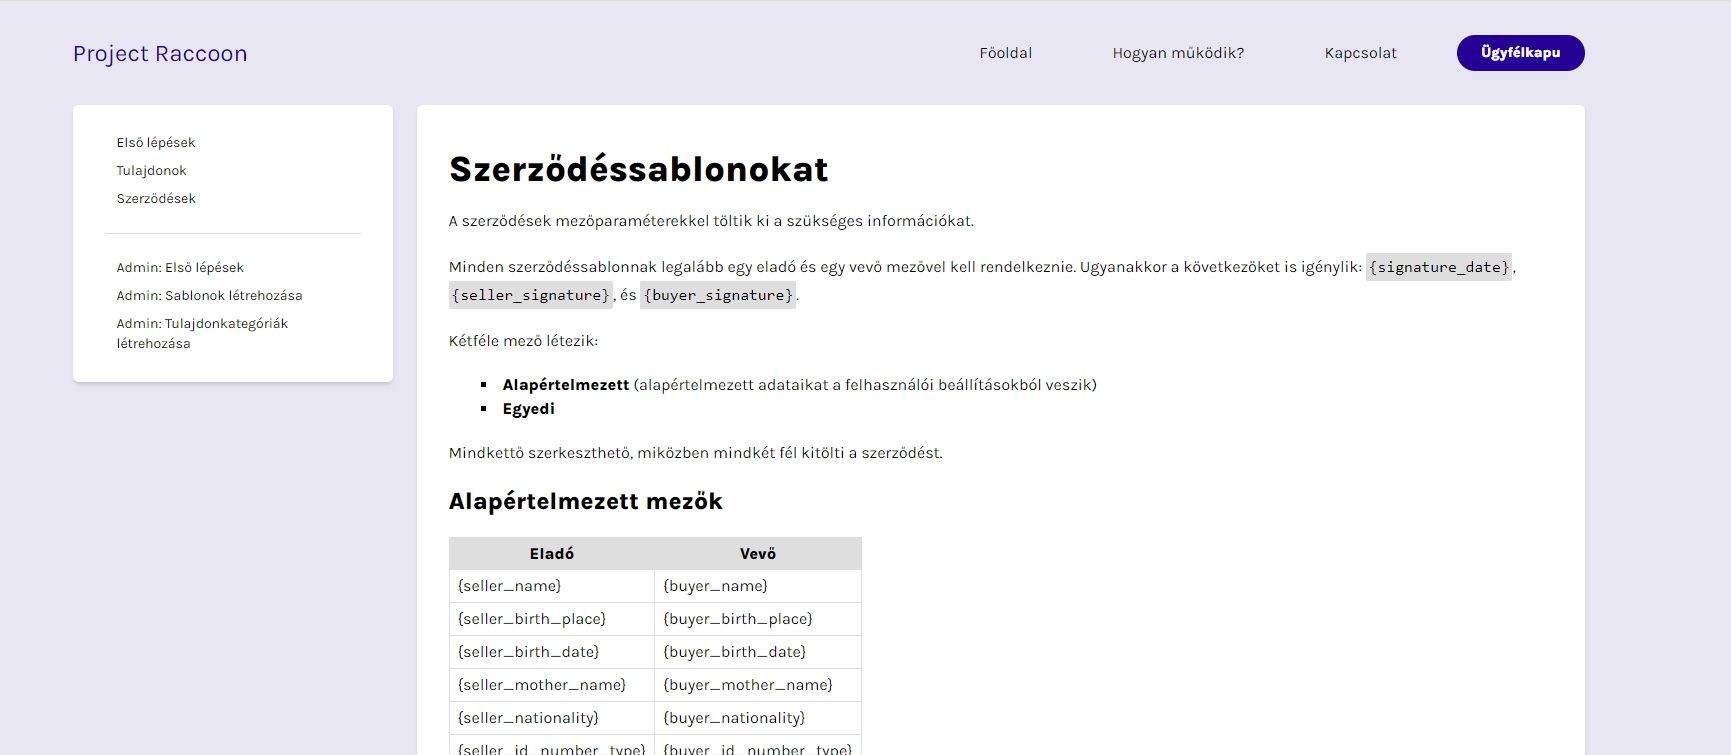
\includegraphics[scale=0.4]{images/design/admin-doc.png}
	\caption{A szerződéssablonok létrehozásának súgója}
        \label{design:adminDoc}
\end{figure}

A súgó, vagyis a menüben ``Dokumentáció''-ként megjelenő menüpont két részre osztódik. Létezik egy az átlagos felhasználók számára, és készült egy az adminisztrátorok számára is. Erre a döntésre azért jutottunk, mert nem szerettük volna az átlagos felhasználók számára is megjeleníteni olyan információkat, amelyeket nem tudnak elérni, tehát használhatatlan lett volna számukra. Így minden, amit megtalálnak a súgóban az releváns és naprakész marad számukra, nem árassza el őket a végtelen/szűretlen információk tárháza. A \ref{design:adminDoc}. ábrán láthatjuk az adminisztrátorok számára készült verzió egyik oldalát, pontosabban a szerződéssablonok létrehozását és magyarázatát. Ezzel kanyarodjuk is át egy fontos témakörhöz, mégpedig ahhoz, hogyan kezeli a Raccoon, és pontosabban hogyan adhatunk hozzá mi szerződéssablonokat, mint adminisztrátorok a portálon. 

A szerződéssablonok feltölthetőek az ``Új szerződés létrehozása'' menüpont alatt (amely megtalálható a navigációs menü admin részén, közvetlenül az előző fejezetben tárgyalt menüpontok alatt). A szerződések mezőparaméterekkel töltik ki a szükséges információkat. Minden szerződéssablonnak legalább egy eladó és egy vevő mezővel kell rendelkeznie. Ugyanakkor a következőket is igénylik: \verb|{signature_date}|, \verb|{seller_signature}|, és \verb|{buyer_signature}|. Kétféle mező létezik:
\begin{itemize}
    \item Alapértelmezett mező (alapértelmezett adataikat a felhasználói beállításokból veszik)
    \item Egyedi mező
\end{itemize}

Alapértelemett mező esetén a következőekre kell gondolni: a vevő, illetve eladó neve, email címe, telefonszáma, személyi igazolvány típusa és száma, születési helyük és idejük stb. A \verb|{signature_date}| egy speciális mező, amely tartalmazza azt a dátumot, amikor a szerződést mindkét fél aláírta. A \verb|{seller_signature}| és a \verb|{buyer_signature}| helyére mind az eladó, mind a vevő neve nagybetűvel kerül. 

Egyedi mezők megadására is lehetőség van, ekkor ezeknek meg kell adni típusát, beírható karakterek hosszát és egyéb esetleges megkötéseket stb a második fázisban. 

A \ref{exampleContract}. ábrán láthatunk egy ilyen példa szerződést, hogy hogyan is nézne ki a mezőkkel.

\begin{figure}[!h]
	\centering
        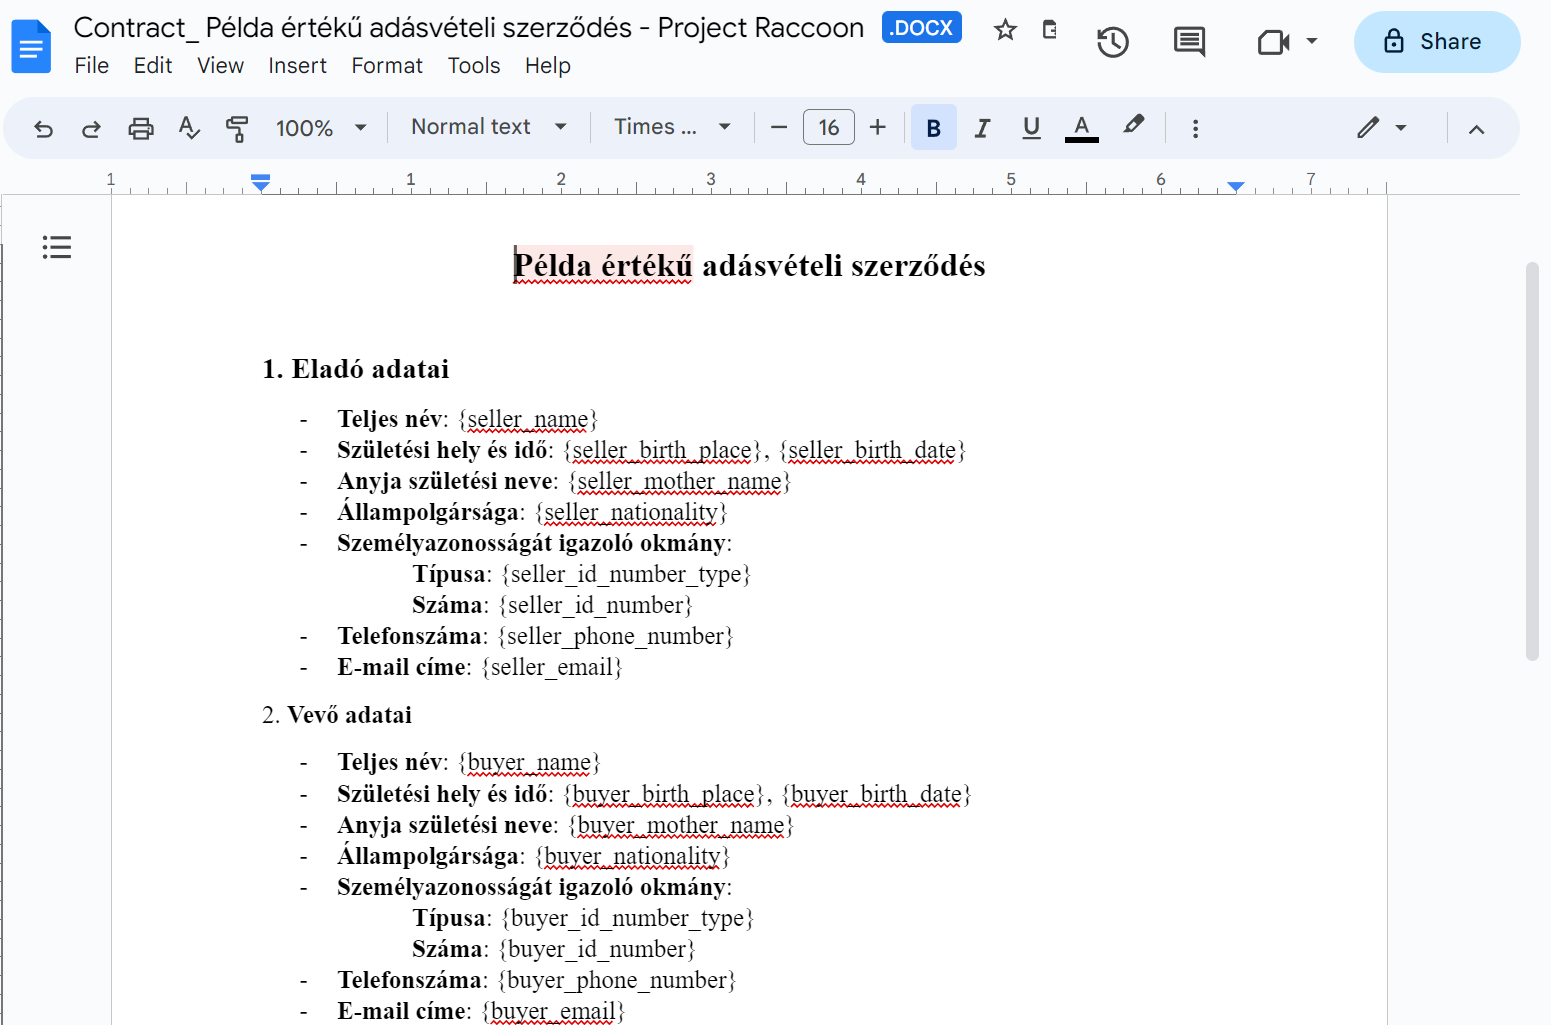
\includegraphics[scale=0.4]{images/design/google-docs.png}
	\caption{Példa értékű adásviteli szerződés szerkesztése Google Docsszal}
        \label{exampleContract}
\end{figure}

Ezen sablondokumentumok szerkeszthetőek Google Docs segítségével, illetve új sablonokat is fel lehet tölteni. 

Egy tényleges új sablon bevezetéséhez szükséges a továbbiakban a platformon megadni a helyettesítési mezőket és azok ``értékeit''. Vagyis miután feltöltöttük a sablont, amely tartalmazza a cserélendő szövegeket a következő formában: \verb|{replacement_option}|, az adminisztrátornak meg kell mondania, hogy ezeket a \{\} közé írt szövegeket a Raccoon mivel helyettesítse. Illetve itt történik a különböző megkötések megadása is, amelyek ezekre a mezőkre érvényesek kell legyenek. 

Összefoglalva tehát a folyamat két lépésből áll: 
\begin{enumerate}
    \item sablon készítése Google Docs-on
    \item helyettesítési mezők megadása a Raccoonon
\end{enumerate}

\begin{figure}[!h]
	\centering
        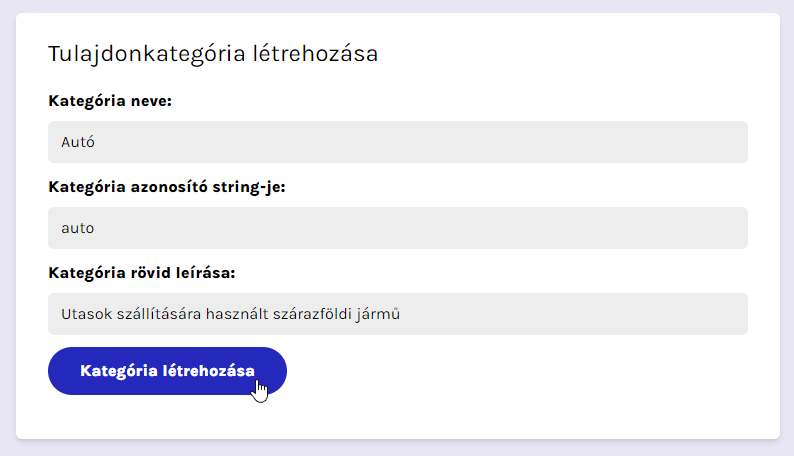
\includegraphics[scale=0.4]{images/design/new-property-category.png}
	\caption{Egy új tulajdonkategória (autó) hozzáadása a Raccoon platformján}
        \label{design:newPropertyCategory}
\end{figure}

Hasonlóképp létrehozhatóak új tulajdonkategóriák is (\ref{design:newPropertyCategory}. ábra). Ebben az esetben egy űrlapot kell kitölteni a Raccoon platformján. Új tulajdonkategória létrehozásához meg kell adnia egy nevet és egy rövid leírást. A kategória azonosítója automatikusan kitöltődik a kategória neve alapján, de szerkeszthető. Az összes korábban létrehozott kategóriát megtekinthetjük a ``Tulajdonkategóriák'' menüpont alatt. Új mezőt is hozzáadhatunk egy meglévő tulajdonkategóriához, ehhez az előbb említett menüben ki kell választani egy, majd megnyomva a ``Kategória szerkesztése'' gombot elénk tárul egy menü, ahol új mezőket adhatunk hozzá a kiválasztott tulajdonkategóriához. A következő paramétereket tudjuk megadni egy ilyen mezőnek: a típusa, prioritása (magasabb prioritás hamarabb jelenik meg), neve, egy hosszabb leírás/magyarázat (nem kötelező), sugó szöveg (nem kötelező), helyettesítő karakterlánc a dokumentumban (ennek a mezőnek a .docx sablonban is szerepelnie kell), minimális hossz (megkötés, nem kötelező), illetve maximális hossz (megkötés, szintén nem kötelező). Ha a hossz helyére $-1$-et írunk, az azt jelenti, hogy a hossz nincs meghatározva. A \ref{design:newPropertyField}. ábrán egy ilyen űrlapot töltöttünk ki egy új mező létrehozására.

\begin{figure}[!h]
	\centering
        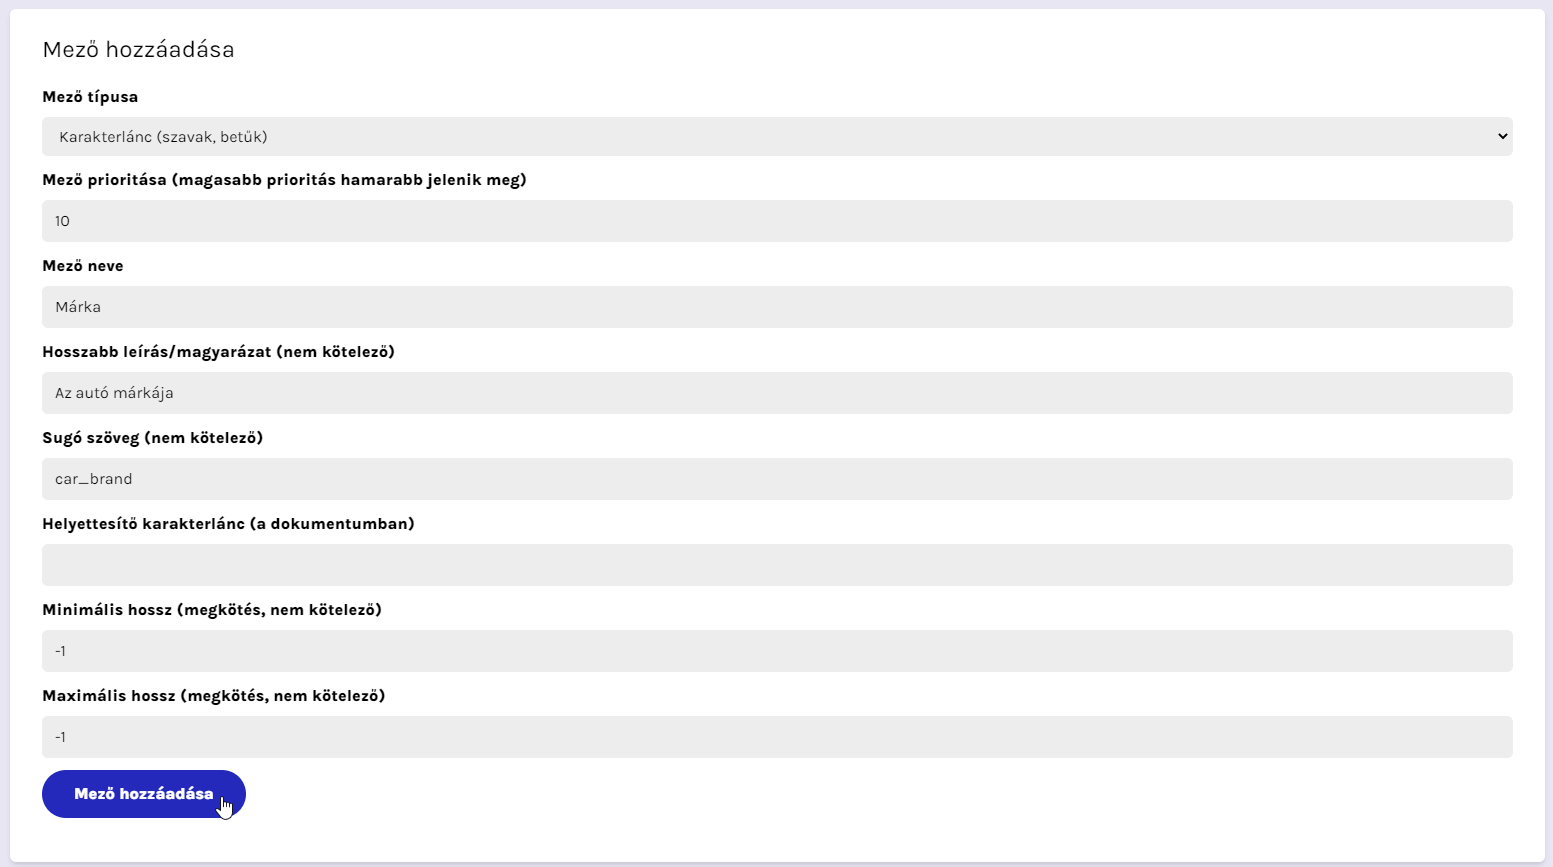
\includegraphics[scale=0.36]{images/design/new-property-field.png}
	\caption{Egy új mező (márka) hozzáadása a Raccoon platformján}
        \label{design:newPropertyField}
\end{figure}

A szerződésekhez lehet ügyvédeket is hozzáadni, az ``Ügyvéd hozzáadása'' menüpont alatt, amely email cím alapján történik. Ezt szintén csak adminisztrátori jogkörrel lehetséges. 

Az átlagfelhasználó számára rendkívül fontos, hogy könnyen áttekinthető módon kezelje szerződéseit és tulajdonait. Az alkalmazás lehetővé teszi számára, hogy listázza az összes szerződését és tulajdonát, amelyekben könnyedén kereshet név vagy típus alapján. 

Az alkalmazás továbbfejlesztésével lehetőséget adhatunk az átlagfelhasználónak arra is, hogy új szerződéseket vigyen be a rendszerbe. Ezáltal egyszerűen rögzítheti és kezelheti új üzleti vagy személyes szerződéseit a platformon keresztül. Az új szerződések felvitelekor a felhasználó részletes információkat adhat meg, például a szerződés leírását, a felek nevét és az érvényességi időtartamot. Ez segíti az átlagfelhasználót abban, hogy a szerződések könnyen azonosíthatók és kezelhetők legyenek.

Az aláírás és letöltés funkció nagyban megkönnyíti az átlagfelhasználó életét. Az alkalmazás lehetővé teszi, hogy a felhasználók elektronikusan aláírják a szerződéseket, így elkerülve a hagyományos papíralapú eljárásokat és a helyhez kötöttséget. Az aláírás után a felhasználók letölthetik a szerződéseket PDF formátumban, így könnyedén megőrizhetik és megoszthatják őket más féllel.

\begin{figure}[!h]
	\centering
        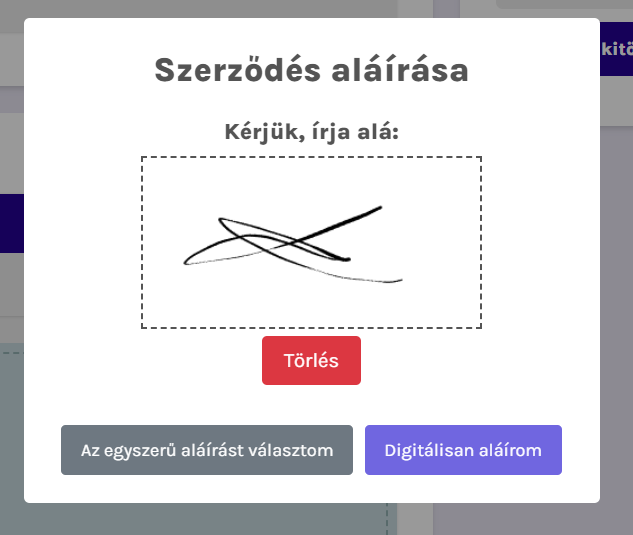
\includegraphics[scale=0.5]{images/design/signature.png}
	\caption{A szerződés digitálisan való aláírásra felhívó ablak}
        \label{design:signature}
\end{figure}

A szerződések aláírása digitális formában történik, erre lehetőséget ad a platform is. Az aláírásra való felkérést a \ref{design:signature}. ábra szemlélteti.

A felhasználók képesek a szerződések mellé csatolmányokat is feltölteni. Erre kényelmes megoldást biztosít az alkalmazás drag-and-drop formájában. Illetve, a felületre rákattintva az operációs rendszer fájlkiválasztó ablakát is megjeleníti. Ez látható a \ref{design:attachment}. ábrán. Abban az esetben, hogyha a felhasználó nem szeretné digitálisan aláírni a szerződést, kiválaszthatja a másik opciót is: az egyszerű aláírás lehetőségét. Az egyszerű aláírás segítségével nem kerül rá konkretán a szerződésre a felhasználó kézírása, helyette a felhasználó neve jelenik meg.

\begin{figure}[!h]
	\centering
        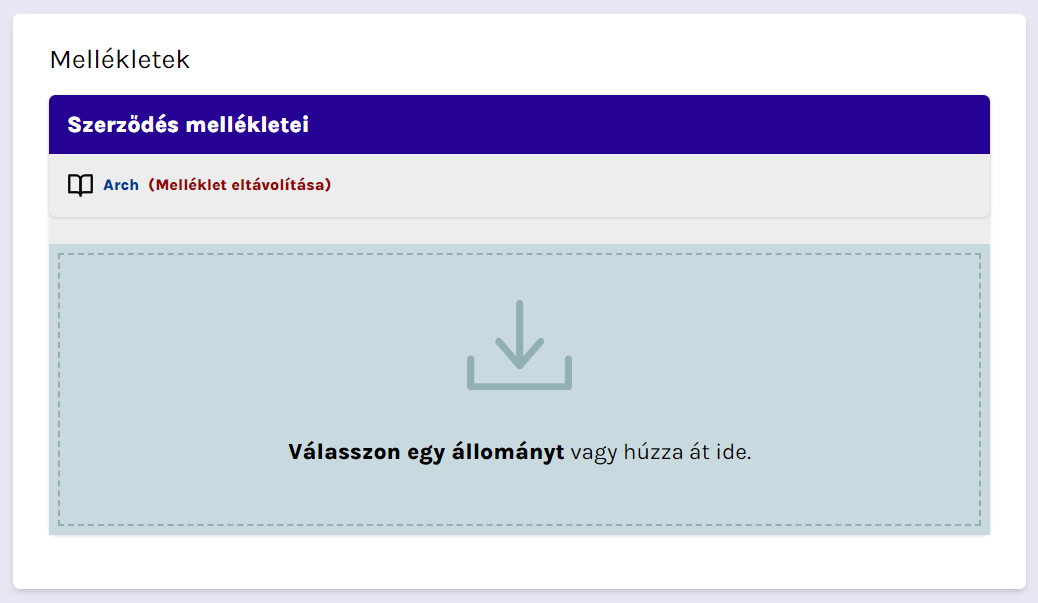
\includegraphics[scale=0.5]{images/design/attachment.png}
	\caption{A szerződésekhez különböző csatolmányokat lehet hozzáadni}
        \label{design:attachment}
\end{figure}

Ezek a fejlesztések hozzájárulnak az alkalmazás hatékonyságához és felhasználóbarát jellegéhez, lehetővé téve az átlagfelhasználó számára, hogy egyszerűen kezelje, keresse és aláírja a szerződéseit, valamint megőrizze fontos tulajdonainak nyilvántartását egy helyen.

Végezetül pedig a weboldalt elláttuk többnyelvűsítéssel is, így a felhasználók könnyedén válthatnak a különböző nyelvek között egy egyszerű kattintással. Ez lehetővé teszi, hogy az alkalmazás használata még inkább személyre szabható legyen, és a felhasználók anyanyelvükön vagy preferált nyelvükön használhassák azt. 

Emellett a platform elérhetővé tette a sötét téma opciót is. Ez lehetővé teszi a felhasználóknak, hogy a hagyományos világos háttér helyett a sötét témát válasszák, ami kevésbé megterhelő a szemüknek és energiatakarékosabb lehet, különösen alacsony fényviszonyok esetén.

Ezek az újítások további funkcionalitást és kényelmet biztosítanak az felhasználók számára, lehetővé téve számukra, hogy könnyedén váltogassanak nyelvek között, és kiválasszák az optimális megjelenést a számukra. Az alkalmazásunk így még rugalmasabbá válik, és az egyéni preferenciákhoz igazodva személyre szabott felhasználói élményt nyújt.